\section{Approach}\label{sec:approach}

\sepfootnotecontent{sf:shapeIndexURL}{
   \ifanonymous
      \url{https://anonymous.4open.science/w/shape-index-specification-707E}
   \else
      \url{https://constraintautomaton.github.io/shape-index-specification/}
   \fi
}

\sepfootnotecontent{sf:recursiveShape}{
    In this paper we ignore ``inverse constraints'' such as
    inverse triple constraint in ShEx 
    %\url{https://shex.io/shex-primer/index.html\#inverse-properties}
    and SHACL Inverse Paths 
    %\url{https://www.w3.org/TR/shacl\#property-path-inverse} 
    to a avoid recurse 
    shape schemas~\cite{Corman2019}.
    We also ignore negative statement.
    We only consider shapes that can be transformed into a single \texttt{SELECT} SPARQL query.
}

\sepfootnotecontent{sf:subwebsep}{
   We assume an implicit conversion between the subweb specification and the formalization of reachability criteria.
   Space constraints prevent us from detailing the conversion.
}

\sepfootnotecontent{sf:ssf_project}{
   The paper \citetitle{delva2023} additional material also proposes a script to convert SCHACL shapes into SPARQL queries.
   \url{https://github.com/MaximeJakubowski/ssf_project}
   \rt{This footnote seems unnecessary, since delva2023 is already cited.}
}


In this section, we first define result-based completeness in LTQP, then formalize the concept of a shape index, a mapping that links RDF data shapes to RDF resources, and finally, describe how the shape index can be used for pruning in LTQP. 


\subsection{Result-Based Completeness in LTQP}\label{sec:slde}

Our approach of pruning in LTQP focus on ensuring result completeness, assuming traversal completeness is already defined using reachability criteria.
By concentrating on result completeness, we explore strategies to optimize the search space of link traversal queries through pruning of irrelevant sources.
We formalize result-based completeness in LTQP as follows.
A query is executed over a DKG $G$ formed by the union of all the $g$ in a network $R$.
The query engine has to build a KG $G^{\prime}$ using a reachability criterion $C^{\prime}$ in its internal data store from the KG $g$ by dereferencing resources $iri \mapsto_{\mathcal{R}} r \in R$.
We formulate an optimization problem to minimize the size of $G^{\prime}$, where the query engine constructs a knowledge graph $G^{\prime\prime} \subseteq G^{\prime}$, potentially smaller, by defining a reachability criterion $C^{\prime\prime}$.
We focus on maintaining the same result completeness, so when using $C^{\prime\prime}$ the following equation must hold

\begin{equation}\label{eq:evalQueryStructuralAssumption}
   [\![ Q ]\!]^{G^{\prime\prime}} = [\![ Q ]\!]^{G^{\prime}}
\end{equation}
for any network $R$.
Since $g \in G^{\prime\prime}$ can only be obtained by dereferencing resources $r \in R$, a smaller $G^\prime$ means fewer HTTP requests were performs to answer a query.  
Generally, query execution is faster with a smaller KG instance, and HTTP requests, being slow and unpredictable~\cite{hartig2016walking}, significantly impact query execution time.  
Thus, reducing HTTP requests provides a twofold benefit.

\subsection{Shape Index}

\iffalse
\begin{figure}
   \centering
   % First figure
   \begin{minipage}[t]{0.45\linewidth}
      \centering
      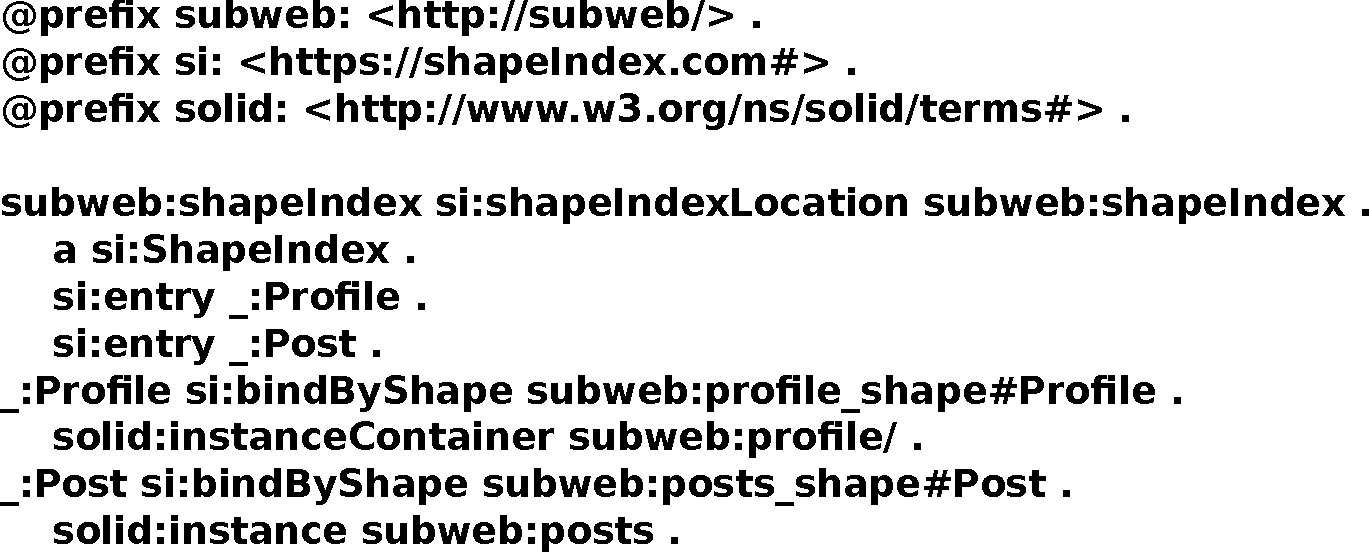
\includegraphics[width=1\textwidth]{figure/shapeIndex.pdf}
      
   \end{minipage}
   %\hspace{0.05\textwidth}
   % Second figure
   \begin{minipage}[t]{0.45\linewidth}
      \centering
      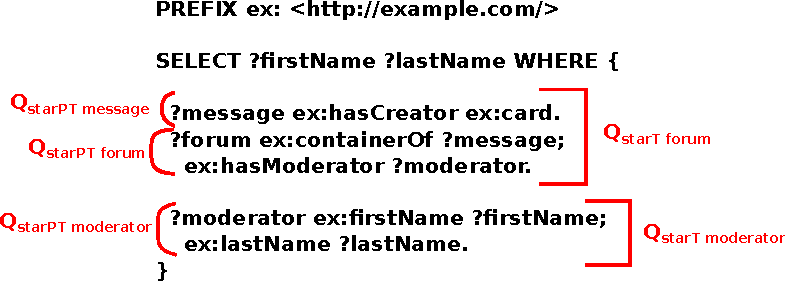
\includegraphics[width=1\textwidth]{figure/q_star.pdf}
   \end{minipage}

   % General caption
   \caption{
      On the left, An example of a shape index mapping a set of IRI to a profile shape and an IRI to a post shape.
       On the right, representation of graph star patterns.
       In red the graph star patterns are presented and in black the partial graph star patterns.
	   \rt{The query does not belong in this example IMO, since the focus is to exemplify the shape index. It may be better to just give some data and document examples matching the shape index. Also, the red labels are never explained AFAICS.}
       }
   \label{fig:shapeIndex}
\end{figure}
\fi

\begin{figure}
   \centering
   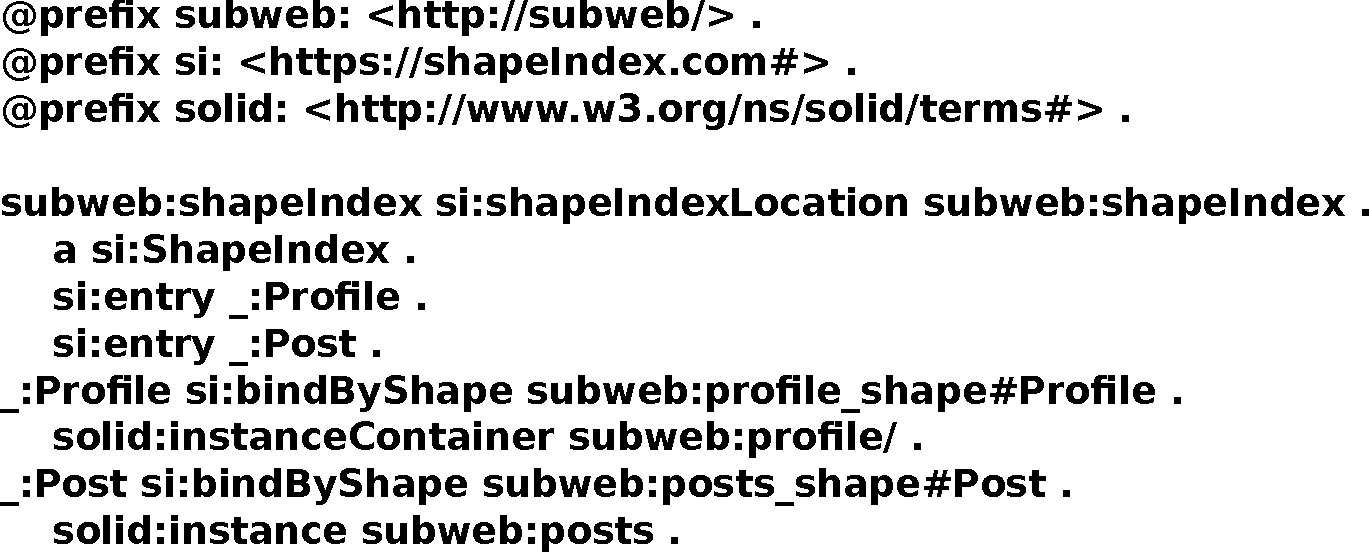
\includegraphics[width=0.5\textwidth]{figure/shapeIndex.pdf}

   \caption{An example of a shape index mapping a set of IRI to a profile shape and an IRI to a post shape.}
   \label{fig:shapeIndex}
\end{figure}

Pruning in LTQP requires knowledge of the data models of dereferenced sources.  
However, obtaining complete, up-to-date, and detailed information for each source in a large decentralized network is impractical.  
To address this, we introduce the \emph{shape index}, a mapping between RDF document sets and RDF data shapes that describes a subweb controlled by a data provider.  
When mapped, the associated KG must conform to the shape.  
Unlike triple statistics, shapes are independent of the KG's size or updates that remain compliant, making them a more cost-effective solution for use cases with stable data models. 

We formalize a shape index as follows:
\begin{equation}\label{eq:shapeIndex}
   SI = \left\{ s_1 \mapsto IRI_1, s_2 \mapsto IRI_2 \cdots, s_n \mapsto IRI_n \right\}
\end{equation}
where $s_i$ is a shape and $IRI_i$ is a set of IRI given $n$ entries.
The subweb described by the index is defined by $D_{SI} = \bigcup_{IRI \in \text{codomain of }(SI)} IRI$.
%A shape index \emph{must} map every resource in $D_{SI}$.
We denote a shape index as \emph{complete} when every shape $s_i \in \text{dom}(SI)$ has a closed world assumption~\cite{Gayo2018b, Gayo2018} (we also refer to them as closed) and \emph{incomplete} otherwise.
A mapping between a shape and a set of IRIs has implications in the distribution of the data in $D_{SI}$.
When a shape $s$ is mapped to an $IRI$, then the KG targeted by the mapping $G = \left\{ g \mid \forall iri \in D_{SI} (iri \mapsto_{\mathcal{R}} r \land r \mapsto_{\mathcal{G}} g) \right\}$ satisfies $s$.
Given that the shape is closed, then every set of triples in the resource mapped to an $iri \in D_{SI}$ respecting the shape must be in a resource mapped to an $iri \in IRI$.
We provide a complete description of the shape index in an online specification~\sepfootnote{sf:shapeIndexURL} and an example of serialization in Figure~\ref{fig:shapeIndex}.

RDF data shapes use \emph{targets} to identify the set of nodes or entities in a KG to validate.  
In this work, we assume all entities in a KG within a document follow the same RDF data shape.  
We call these entities graph star(s) (patterns), an extension of the RDF star patterns concept~\cite{Karim2020}.  
Defined in Definition~\ref{def:starPattern}, graph stars serve two purposes:
defining targets for validation and capturing relationships between triple patterns and shape entities.  
Star patterns consist of triples with the same subject.
We extend this by linking star patterns where the objects of the triples in one star pattern are the subjects of another, forming a graph structure.
For example, a user linking to their posts with recursive replies can be captured with a root star pattern for the user and nested patterns for the posts and replies.  
Thus, the target of the shapes in the shape index correspond to the subject of each root star pattern when a KG is divided into graph stars with no shared partial graph stars.  
%Figure~\ref{fig:shapeIndex} illustrates an example of a graph star pattern.


\begin{definition}[Graph Star Pattern (GSP)]\label{def:starPattern}
   We define a star pattern $Q_{star}$ as a set of $tp \in Q$~\cite{Karim2020} with the same subject such that 
   given a builder function 
   \begin{equation}
       BQ_{star}(s) = \left\{ tp_i \in Q \mid S(tp_i) = s \right\}
   \end{equation}
   with $s \in \mathcal{I} \cup \mathcal{B} \cup \mathcal{V}$ then $Q_{star_s} = BQ_{star}(s)$.
   We define a GSP $Q_{starT}$ as the union between a root star pattern $Q_{star_s}$
   and the star patterns having as subject term an object term of another star pattern in $Q_{starT}$.
   We define a function 
   $O_{star}: q \in Q \rightarrow  \mathcal{I} \cup \mathcal{B} \cup \mathcal{V}$
   that returns every non-literal object terms of a star pattern.

   We then define $Q_{starT}$ given a  set of partial GSP $Q_{starPT}$
   \begin{equation}
      Q_{starT} = \bigcup_{q \in Q_{starPT}} q
   \end{equation}
   where $Q_{starPT}$ is formed with a root $Q_{star_s}$ by

   \begin{equation}
           Q_{starPT_i} =
       \begin{cases}
         \left\{ Q_{star_s} \right\} & \text{if } i = 1 \\
           \left\{ BQ_{star}(o) \mid o \in \bigcup_{q \in Q_{starPT_{i-1}}} O_{star}(q) \right\} & \text{if } i>1
       \end{cases}
   \end{equation}

   We also define a function  
   $S_{star}: q \rightarrow  \mathcal{I} \cup \mathcal{B} \cup \mathcal{V}$
   returning the subjects of the $Q_{starPT_i}$ of a $Q_{starT}$.

   We propose a similar definition for the context of KGs where we replace the query $Q$ by a KG $G$ and where the terms 
   cannot be a $v \in \mathcal{V}$. 
   We denote this structure a graph star.
   
\end{definition}

The construction and maintenance of shape indexes are beyond the scope of this work.
While not evaluated, shape indexes appear to require less effort to generate than VoID descriptions~\cite{Boehm2011}, as they do not include detailed statistics such as triple counts.
Nonetheless, VoID descriptions have been successfully used for query optimization in federated queries~\cite{Montoya2017}.
RDF data shapes can be either prescriptive or descriptive.
For shape indexes with descriptive shapes, automatic RDF data shape generation methods~\cite{fernandez2023extracting} could facilitate their creation.
Entries in shape indexes correspond to sets of IRIs, which could be structured using URI templates, thereby reducing the need for exhaustive redefinition.
For prescriptive shapes, contributions in shape-based data integration~\cite{LabraGayo2023} could help prevent the generation of invalid data sources.


\subsection{Link Pruning Using Shape Indexes}\label{sec:sourceSelection}

In this section we make the link between the shape index and link pruning in LTQP.
A DKG exposing a shape index provides a query engine with the opportunity to reduce its search domain by knowing which resources are query-relevant.
More formally, instead of traversing the whole DKG $D$ associated with a shape index, the engine will traverse a DKG $D^{\prime} \subseteq D$, ignoring the knowable query-irrelevant sources.
%The concept of composite reachability criteria allows us to ignore certain sources during traversal based on the knowledge acquired during traversal.
Our approach involves dynamically constructing new reachability criteria during traversal that are more selective as we discover and analyze shape indexes.
These criteria are designed so that they will always produce the same completeness of results as the one that was defined at the beginning of the traversal.

\iffalse
\rt{I still think introducing time here is a really bad idea. I'm almost certain that reviewers will shoot the paper down because of this. In the formalization, let's just assume prior knowledge of all shape indexes and corresponding reachability criteria. Combining them during query execution is an implementation detail.}
More formally, let us introduce time $t$ as a factor for our reachability criteria $C_t$.
The query execution begins with an initial reachability criterion $C_0$.
At any time $t$, Equation~\ref{eq:evalQueryStructuralAssumption} must hold if we consider $C_t = C_{t+1} = C_{t+2} \dots = C_{tf}$ until the end of the execution $tf$, given that $G^{\prime}$ is produced using $C_0$.
\fi

To define more selective reachabilities, we propose extending the reachability criteria by formalizing a chain of criteria in a concept called \emph{composite reachability criteria}.
In this form, a reachability criterion $cp_i$ is said to \emph{prune} links, and $cd_i$ is said to \emph{discover} links.
Equation~\ref{eq:cReachabilityCriteria} formalizes a composite reachability criterion $C$.
where $Cd$ is the set of every $cd_i(t, iri, Q)$ and $Cp$ the set of every $cp_i(t, iri, Q)$ used by the engine.

\begin{equation}\label{eq:cReachabilityCriteria}
   C(t, iri, Q) = \bigvee_{cd \in Cd} cd(t, iri, Q) \mathrel{\land} \bigwedge_{cp \in Cp} \, cp(t, iri, Q)
\end{equation}

To perform pruning in LTQP with shape indexes, an initial reachability criterion $C_0$ is defined.
This criterion must include a discovery reachability criterion $cd_{\text{shape index}}$ that leads to a shape index document.  
After dereferencing a shape index $SI_i$, the query engine creates a set of links $IRI_p$ containing the links to prune.  
The links to prune are identified by evaluating the shape index to find IRIs that are not relevant to the query, such that Equation~\ref{eq:evalQueryStructuralAssumption} holds, given that $G^{\prime}$ is produced using $C_0$.  
This is done by performing a query-shape subsumption check ($\sqsubseteq_{qs}$), defined later in Section~\ref{sec:containment}.

We define
$IRI_p = \left\{ \bigcup SI_i(s_j) | s_j \sqsubseteq_{qs}  Q = \mathrm{false} \land s_j \in \text{dom}(SI_i) \right\}$.
From this sets of links we define a pruning reachability criteria;
\begin{equation}
       cp_{si}(t, iri, Q) = iri \notin IRI_p
\end{equation}
The new reachability $C^{\prime\prime}_i$ is created by taking the $Cd$ and $Cp$ of $C^{\prime\prime}_{i-1}$ and adding
and $cp_{si}$ to $Cp$.

This approach has three main limitations.  
First, it assumes that data providers maintain up-to-date shape indexes; outdated indexes may lead to incomplete results.
A similar criticism could be made against the method exploiting VoID descriptions~\cite{Montoya2017}.
Second, if the query-shape subsumption check requires dereferencing all documents, it becomes ineffective and may slow down query execution.  
Third, the approach does not consider cases where querying irrelevant documents could uncover relevant ones via additional reachability criteria.  
Addressing this would require translating these criteria into queries, which is beyond the scope of this paper.

\subsection{Query-Shape Subsumption}\label{sec:containment}
To determine whether the content of a resource conforming to a shape is query-relevant, a \emph{query-shape subsumption} problem is solved.  
This problem is analogous to the query subsumption problem which is a weaker form of the classic query containment problem~\cite{Spasi2023}.
Query containment asses whether a query can be answered from the answer of another query,  independent to the database or KG~\cite{afariQCE}.
In the subsumption problem a sub query $Q1$ is subsumed by a super query $Q2$  if every result of $Q1$ can be extended to a result of $Q2$ for any database~\cite{Spasi2023, Pichler2014}.
In our approach to query-shape subsumption, we aim to determine whether a GSP in a query can be answered by evaluating any source conforming to a specific shape.
Thus, we differ from the standard subsumption problem, as the solution mappings of the super query $Q_2$ must be extended to answer $Q_1$.
It is a common approach for shape validation over an RDF graph to convert shapes into SPARQL queries~\cite{labragayo2017validatingdescribinglinkeddata, Corman2019,Prestamo2023, spapeExpressionConvert}.~\sepfootnote{sf:recursiveShape}
We refer to this transformation of a shape $s$ as $T(s)$ producing a query $Q_s$.
We consider shapes with open world assumption to always represent queries that retrieve entire KGs.
This is because, under the open-world assumption, a shape defines the minimum constraints of a graph.

Query subsumption may initially seem unsuitable for dynamic reachability due to its $\Pi^P_2$ time complexity~\cite{Pichler2014, Letelier2013}.  
However, this complexity depends on the size of the queries, which are typically small in practice~\cite{Doan2012}.  
In most cases, queries do not contain thousands or millions of triple patterns~\cite{Bonifati2019}.  
%Furthermore, practical use cases can often take advantage of polynomial-time algorithms~\cite{Doan2012}.
Additionally, as mentioned earlier, we are not addressing a standard subsumption problem, and analyzing its general complexity is beyond the scope of this paper.
In our context, the sub query adheres to a GSP template structure, where predicates are always IRIs.
This structure arises because shapes predominantly describe predicate terms and object terms and are isomorphic to the specific KG.
By exploiting this structure, it is possible to design an algorithm with polynomial time complexity.

We consider that a shape $S$ is subsumed by a query $Q$ denoted as $S \sqsubseteq_{qs} Q$, 
if for any KG $G_s$ respecting the shape there is a GSP in $Q$ that can find a solution.
For a GSP to subsumed $S$, we need to consider $Q$ and $Q_s$ to have the two parts $Q = Q_{\text{body}} \bowtie Q_{\text{unions}}$.
$Q_{\text{body}}$ is the Basic Graph Pattern (BGP) of the query, and $Q_{\text{unions}} = \bigcup Q_u$ represents the Union Graph Patterns (UGP)~\cite{w3SPARQLQuery}, where $Q_u = q_0 \cup q_1$.
We assume that $q_i$ have no union statement.
\iffalse
A graph star pattern $Q_{\text{starT}_i}$ is contained in $Q_s$ if its segment in $Q_{\text{body}}$ is contained in $Q_s$, and if its segment in at least one $q_i$ in each $Q_u$ is contained in $Q_s$. 
If $Q_{\text{starT}_i}$ is not part of any $Q_u$, then $Q_u$ is ignored.
\fi
\iffalse
For the simplicity of the formalization we ignore other SPARQL operators such has \texttt{GROUP BY} and Filter expressions,
however given query-shape subsumption  is transformed into query containment problem there are methods in the litterature to handle a more complete SPARQL fragment~\cite{Spasi2023}.
\fi

\iffalse
\rt{I would not mention everything after this, and instead at the start of this paragraph say that for simplicity of this formalization, we focus on just BGPs of triple patterns and unions.}
In our containment problem, we ignore \texttt{GROUP BY} segments.
We make this choice because, in the context of shape queries, \texttt{GROUP BY} is primarily used to set a cardinality, and we are not attempting to identify sources that can fully answer specific segments of a query. 
Instead, our goal is to disregard data sources that are irrelevant to the query, given the constraints imposed by the shape index. 
Discriminating based on cardinalities could potentially affect query results.
Additionally, this article does not consider filter expressions, as they can significantly increase the complexity of the problem.
Moreover, "false" negatives do not impact the correctness of our approach. \rt{But this is important to mention indeed! But needs some more elaboration on the fact that doing more (useless) requests is not a problem.}
However, incorporating filter expressions into future work would be an interesting direction to explore.
\fi
% https://en.wikipedia.org/wiki/Master_theorem_(analysis_of_algorithms)
\begin{algorithm}[h]
   \caption{Check if a GSP subsumes a $Q_s$ ($subsums_{\text{graph star}}$)}\label{alg:containmentTree}
   \begin{algorithmic}
      \algsetup{linenosize=\tiny}
      \scriptsize

      \REQUIRE  $Q_{star}$, $Q_{starT_i}$, $Q_s = Q_{s\text{body}} \cup Q_{s\text{unions}}$ and $Eval_{star}$
      \ENSURE \TRUE $ $ or \FALSE $ $ whether the root of a graph star pattern $Q_{star}$ is contained in the shape.

      \IF{$S_{star}(Q_{star}) \in Eval_{star}$}
         \RETURN \TRUE
      \ENDIF 

      \FORALL{$tp \in Q_{star}$} % O(n_star)
         \IF{\NOT $match(tp, Q_{s\text{body}})$}
            \STATE $hasOnePath \gets $ \FALSE
            \FORALL{$q_{us} \in Q_{s\text{unions}}$}
               \IF{$subsums_{\text{graph star}}(Q_{star}, Q_{starT_i}, q_{us}, Eval_{star})$}
                  \STATE $hasOnePath \gets $ \TRUE
               \ENDIF
            \ENDFOR
            \IF{\NOT $hasOnePath$}
               \RETURN \FALSE
            \ENDIF
         \ELSE
            %eval nested
            \IF{$O(tp) \in  S_{star}(Q_{starT_i})$}
               \IF{\NOT $subsums_{\text{graph star}}(Q_{star_{O(tp)}} \in Q_{starT_i}, Q_{starT_i}, Q_s, Eval_{star})$}
                  \RETURN \FALSE
               \ENDIF
            \ENDIF
            %
         \ENDIF
      \ENDFOR

      \STATE $Eval_{star} \gets Eval_{star} \cup S_{star}(Q_{star})$
      \RETURN \TRUE
   \end{algorithmic}
\end{algorithm}


We define the function $subsums_{\text{graph star}}$ in Algorithm~\ref{alg:containmentTree} to evaluate whether a GSP with a root star pattern $Q_{star_i}$ from $Q_{starT_i}$ sumbsumes $Q_s$. 
The algorithm also takes a set $Eval_{star}$ to track which partial graph star patterns have already been evaluated.
The algorithm works by examining each triple pattern in the root star pattern $Q_{star_i}$ and checking if an equivalent triple pattern (ignoring the variable names) can be found in the BGP of $Q_s$ using the $match$ function.
If the triple pattern cannot be found in the BGP, the algorithm then looks into the UGPs of $Q_s$. 
Since we assume that the union statements are not nested, this limits the number of recursive calls.
If an equivalent triple pattern is found, the algorithm checks whether the object of the triple pattern is the subject of a partial graph star pattern in $Q_{starT_i}$.
If it is, the algorithm recursively applies the same procedure to this partial graph star pattern as $Q_{star_i}$.
To avoid cycles and redundant evaluations when processing the object of the star patterns, we maintain a set of evaluated subjects in $Eval_{star}$.
We notice that the complexity of Algorithm~\ref{alg:containmentTree} is $O(n_{tp} \times n_{sunion})$
where $n_{tp}$ is the number of triple patterns of $Q_{starT_i}$ and $n_{sunion}$ the number of UGP in $Q_s$.
To solve $S \sqsubseteq_{qs} Q$, we need to consider the number of GSP from the BGP with their number of segments in the UGP and the number of BGPs in the UGPs.
This operation results again in a polynomial time complexity algorithm.
%To solve $Q \sqsubseteq_{qs} S$, we need to consider the $n_{starT}$ graph star from the BGP with their $n_{starTu}$ segment in the UGP and $n_{starTui}$ BGP in the UGP.
%This operation results in a polynomial time complexity of $O(n_o \times n_{tp}^2 \times n_{union}^2 \times n_{starT} \times n_{starTu} \times n_{starTui})$.
%In the \nameref{sec:appendix} Algorithm~\ref{alg:containment} present the full resolution to evaluate each graph star pattern.
